\documentclass{standalone}
\usepackage{tikz}
\usetikzlibrary{patterns, positioning}

\begin{document}
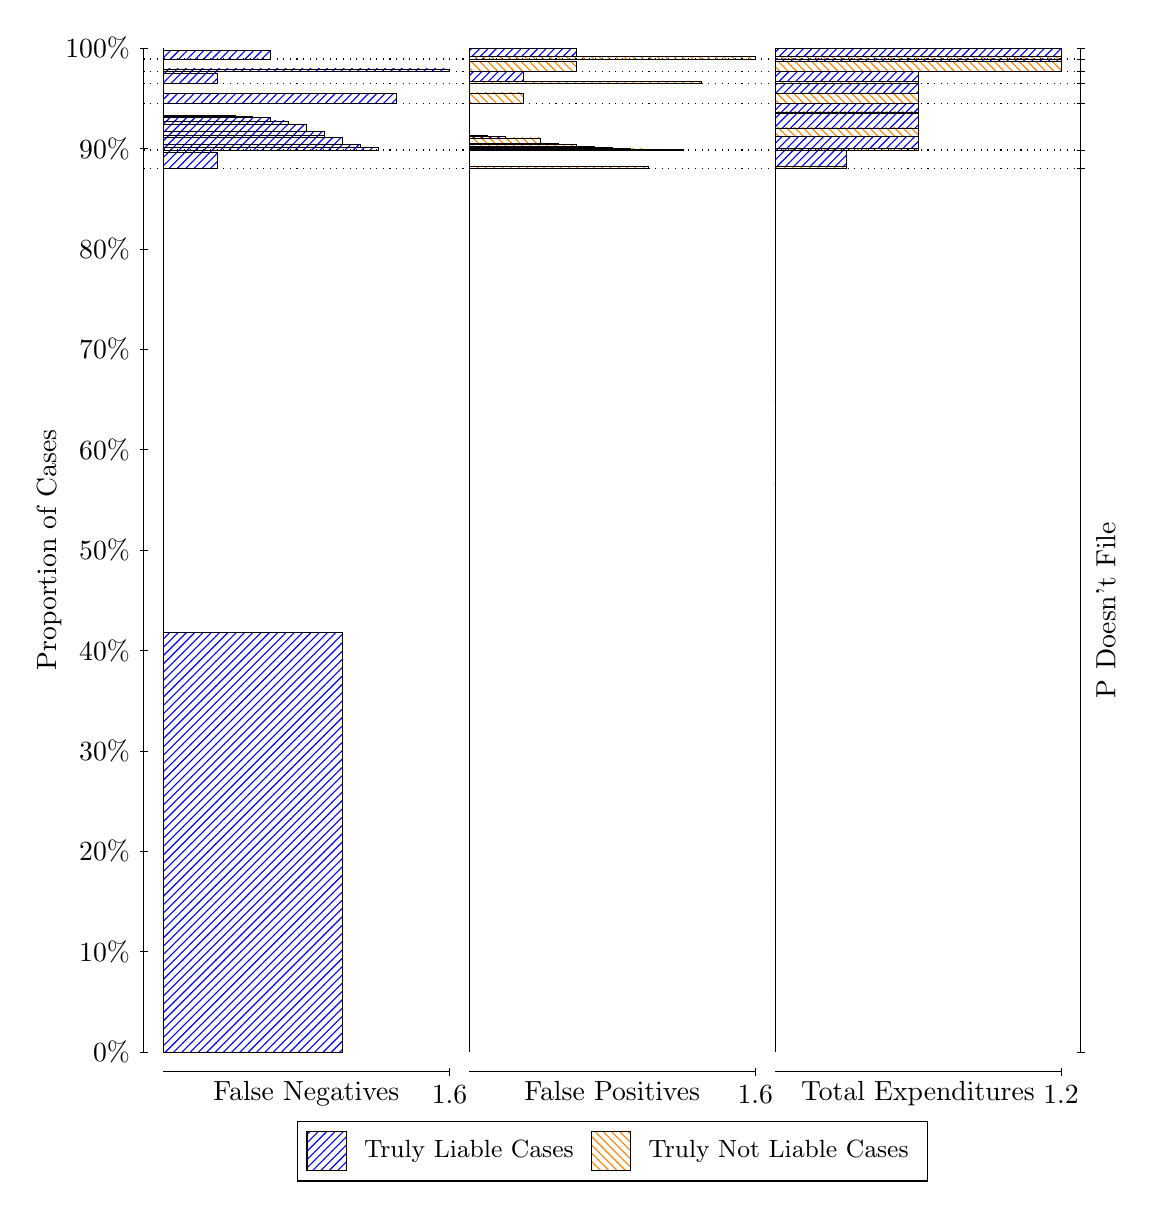
\begin{tikzpicture}
\draw[black, very thin] (1.5,1.75) -- (1.5,14.5);
\node[rotate=90, anchor=center] at (0.3, 8.125) {Proportion of Cases};
\draw[black, very thin] (1.45,1.75) -- (1.55,1.75);
\node[anchor=east] at (1.45, 1.75) {0\%};
\draw[black, very thin] (1.45,3.025) -- (1.55,3.025);
\node[anchor=east] at (1.45, 3.025) {10\%};
\draw[black, very thin] (1.45,4.3) -- (1.55,4.3);
\node[anchor=east] at (1.45, 4.3) {20\%};
\draw[black, very thin] (1.45,5.575) -- (1.55,5.575);
\node[anchor=east] at (1.45, 5.575) {30\%};
\draw[black, very thin] (1.45,6.85) -- (1.55,6.85);
\node[anchor=east] at (1.45, 6.85) {40\%};
\draw[black, very thin] (1.45,8.125) -- (1.55,8.125);
\node[anchor=east] at (1.45, 8.125) {50\%};
\draw[black, very thin] (1.45,9.4) -- (1.55,9.4);
\node[anchor=east] at (1.45, 9.4) {60\%};
\draw[black, very thin] (1.45,10.675) -- (1.55,10.675);
\node[anchor=east] at (1.45, 10.675) {70\%};
\draw[black, very thin] (1.45,11.95) -- (1.55,11.95);
\node[anchor=east] at (1.45, 11.95) {80\%};
\draw[black, very thin] (1.45,13.225) -- (1.55,13.225);
\node[anchor=east] at (1.45, 13.225) {90\%};
\draw[black, very thin] (1.45,14.5) -- (1.55,14.5);
\node[anchor=east] at (1.45, 14.5) {100\%};

\draw[black, very thin] (13.4,1.75) -- (13.4,14.5);
\draw[black, very thin] (13.35,1.75) -- (13.45,1.75);
\node[anchor=west] at (13.35, 1.75) {};
\draw[black, very thin] (13.35,12.973) -- (13.45,12.973);
\node[anchor=west] at (13.35, 12.973) {};
\draw[black, very thin] (13.35,13.205) -- (13.45,13.205);
\node[anchor=west] at (13.35, 13.205) {};
\draw[black, very thin] (13.35,13.799) -- (13.45,13.799);
\node[anchor=west] at (13.35, 13.799) {};
\draw[black, very thin] (13.35,14.05) -- (13.45,14.05);
\node[anchor=west] at (13.35, 14.05) {};
\draw[black, very thin] (13.35,14.204) -- (13.45,14.204);
\node[anchor=west] at (13.35, 14.204) {};
\draw[black, very thin] (13.35,14.361) -- (13.45,14.361);
\node[anchor=west] at (13.35, 14.361) {};
\draw[black, very thin] (13.35,14.5) -- (13.45,14.5);
\node[anchor=west] at (13.35, 14.5) {};

\draw[black, very thin, pattern color=blue, pattern=north east lines] (1.75,1.75) rectangle (4.0208,7.0801);
\draw[black, very thin, pattern color=orange, pattern=north west lines] (1.75,7.0801) rectangle (1.75,12.973);
\draw[black, very thin, pattern color=blue, pattern=north east lines] (1.75,12.973) rectangle (2.4312,13.182);
\draw[black, very thin, pattern color=orange, pattern=north west lines] (1.75,13.182) rectangle (1.75,13.205);
\draw[black, very thin, pattern color=blue, pattern=north east lines] (1.75,13.205) rectangle (4.475,13.24);
\draw[black, very thin, pattern color=blue, pattern=north east lines] (1.75,13.24) rectangle (4.2479,13.277);
\draw[black, very thin, pattern color=blue, pattern=north east lines] (1.75,13.277) rectangle (4.0208,13.364);
\draw[black, very thin, pattern color=blue, pattern=north east lines] (1.75,13.364) rectangle (3.7937,13.391);
\draw[black, very thin, pattern color=blue, pattern=north east lines] (1.75,13.391) rectangle (3.7937,13.442);
\draw[black, very thin, pattern color=blue, pattern=north east lines] (1.75,13.442) rectangle (3.5667,13.534);
\draw[black, very thin, pattern color=blue, pattern=north east lines] (1.75,13.534) rectangle (3.3396,13.576);
\draw[black, very thin, pattern color=blue, pattern=north east lines] (1.75,13.576) rectangle (3.1125,13.616);
\draw[black, very thin, pattern color=blue, pattern=north east lines] (1.75,13.616) rectangle (2.8854,13.63);
\draw[black, very thin, pattern color=blue, pattern=north east lines] (1.75,13.63) rectangle (2.6583,13.646);
\draw[black, very thin, pattern color=orange, pattern=north west lines] (1.75,13.646) rectangle (1.75,13.799);
\draw[black, very thin, pattern color=blue, pattern=north east lines] (1.75,13.799) rectangle (4.7021,13.919);
\draw[black, very thin, pattern color=orange, pattern=north west lines] (1.75,13.919) rectangle (1.75,14.05);
\draw[black, very thin, pattern color=blue, pattern=north east lines] (1.75,14.05) rectangle (2.4312,14.183);
\draw[black, very thin, pattern color=orange, pattern=north west lines] (1.75,14.183) rectangle (1.75,14.204);
\draw[black, very thin, pattern color=blue, pattern=north east lines] (1.75,14.204) rectangle (5.3833,14.236);
\draw[black, very thin, pattern color=orange, pattern=north west lines] (1.75,14.236) rectangle (1.75,14.361);
\draw[black, very thin, pattern color=blue, pattern=north east lines] (1.75,14.361) rectangle (3.1125,14.471);
\draw[black, very thin, pattern color=orange, pattern=north west lines] (1.75,14.471) rectangle (1.75,14.5);
\draw[black, very thin, pattern color=orange, pattern=north west lines] (5.6333,1.75) rectangle (5.6333,7.6426);
\draw[black, very thin, pattern color=blue, pattern=north east lines] (5.6333,7.6426) rectangle (5.6333,12.973);
\draw[black, very thin, pattern color=orange, pattern=north west lines] (5.6333,12.973) rectangle (7.9042,12.996);
\draw[black, very thin, pattern color=blue, pattern=north east lines] (5.6333,12.996) rectangle (5.6333,13.205);
\draw[black, very thin, pattern color=orange, pattern=north west lines] (5.6333,13.205) rectangle (8.3583,13.208);
\draw[black, very thin, pattern color=orange, pattern=north west lines] (5.6333,13.208) rectangle (8.1313,13.211);
\draw[black, very thin, pattern color=orange, pattern=north west lines] (5.6333,13.211) rectangle (7.9042,13.218);
\draw[black, very thin, pattern color=orange, pattern=north west lines] (5.6333,13.218) rectangle (7.6771,13.225);
\draw[black, very thin, pattern color=orange, pattern=north west lines] (5.6333,13.225) rectangle (7.45,13.24);
\draw[black, very thin, pattern color=orange, pattern=north west lines] (5.6333,13.24) rectangle (7.2229,13.251);
\draw[black, very thin, pattern color=orange, pattern=north west lines] (5.6333,13.251) rectangle (6.9958,13.276);
\draw[black, very thin, pattern color=orange, pattern=north west lines] (5.6333,13.276) rectangle (6.7687,13.293);
\draw[black, very thin, pattern color=orange, pattern=north west lines] (5.6333,13.293) rectangle (6.5417,13.358);
\draw[black, very thin, pattern color=blue, pattern=north east lines] (5.6333,13.358) rectangle (6.0875,13.375);
\draw[black, very thin, pattern color=blue, pattern=north east lines] (5.6333,13.375) rectangle (5.8604,13.388);
\draw[black, very thin, pattern color=blue, pattern=north east lines] (5.6333,13.388) rectangle (5.6333,13.799);
\draw[black, very thin, pattern color=orange, pattern=north west lines] (5.6333,13.799) rectangle (6.3146,13.93);
\draw[black, very thin, pattern color=blue, pattern=north east lines] (5.6333,13.93) rectangle (5.6333,14.05);
\draw[black, very thin, pattern color=orange, pattern=north west lines] (5.6333,14.05) rectangle (8.5854,14.072);
\draw[black, very thin, pattern color=blue, pattern=north east lines] (5.6333,14.072) rectangle (6.3146,14.204);
\draw[black, very thin, pattern color=orange, pattern=north west lines] (5.6333,14.204) rectangle (6.9958,14.329);
\draw[black, very thin, pattern color=blue, pattern=north east lines] (5.6333,14.329) rectangle (5.6333,14.361);
\draw[black, very thin, pattern color=orange, pattern=north west lines] (5.6333,14.361) rectangle (9.2667,14.39);
\draw[black, very thin, pattern color=blue, pattern=north east lines] (5.6333,14.39) rectangle (6.9958,14.5);
\draw[black, very thin, pattern color=orange, pattern=north west lines] (9.5167,1.75) rectangle (9.5167,7.6426);
\draw[black, very thin, pattern color=blue, pattern=north east lines] (9.5167,7.6426) rectangle (9.5167,12.973);
\draw[black, very thin, pattern color=orange, pattern=north west lines] (9.5167,12.973) rectangle (10.425,12.996);
\draw[black, very thin, pattern color=blue, pattern=north east lines] (9.5167,12.996) rectangle (10.425,13.205);
\draw[black, very thin, pattern color=orange, pattern=north west lines] (9.5167,13.205) rectangle (11.333,13.229);
\draw[black, very thin, pattern color=blue, pattern=north east lines] (9.5167,13.229) rectangle (11.333,13.375);
\draw[black, very thin, pattern color=orange, pattern=north west lines] (9.5167,13.375) rectangle (11.333,13.486);
\draw[black, very thin, pattern color=blue, pattern=north east lines] (9.5167,13.486) rectangle (11.333,13.672);
\draw[black, very thin, pattern color=orange, pattern=north west lines] (9.5167,13.672) rectangle (11.333,13.69);
\draw[black, very thin, pattern color=blue, pattern=north east lines] (9.5167,13.69) rectangle (11.333,13.799);
\draw[black, very thin, pattern color=orange, pattern=north west lines] (9.5167,13.799) rectangle (11.333,13.93);
\draw[black, very thin, pattern color=blue, pattern=north east lines] (9.5167,13.93) rectangle (11.333,14.05);
\draw[black, very thin, pattern color=orange, pattern=north west lines] (9.5167,14.05) rectangle (11.333,14.072);
\draw[black, very thin, pattern color=blue, pattern=north east lines] (9.5167,14.072) rectangle (11.333,14.204);
\draw[black, very thin, pattern color=orange, pattern=north west lines] (9.5167,14.204) rectangle (13.15,14.329);
\draw[black, very thin, pattern color=blue, pattern=north east lines] (9.5167,14.329) rectangle (13.15,14.361);
\draw[black, very thin, pattern color=orange, pattern=north west lines] (9.5167,14.361) rectangle (13.15,14.39);
\draw[black, very thin, pattern color=blue, pattern=north east lines] (9.5167,14.39) rectangle (13.15,14.5);
\draw[black, dotted] (1.5,12.973) -- (13.4,12.973);
\draw[black, dotted] (1.5,13.205) -- (13.4,13.205);
\draw[black, dotted] (1.5,13.799) -- (13.4,13.799);
\draw[black, dotted] (1.5,14.05) -- (13.4,14.05);
\draw[black, dotted] (1.5,14.204) -- (13.4,14.204);
\draw[black, dotted] (1.5,14.361) -- (13.4,14.361);
\draw[black, very thin] (1.75,1.5) -- (5.3833,1.5);
\node[anchor=north] at (3.5667, 1.5) {False Negatives};
\draw[black, very thin] (5.3833,1.45) -- (5.3833,1.55);
\node[anchor=north] at (5.3833, 1.45) {1.6};

\draw[black, very thin] (5.6333,1.5) -- (9.2667,1.5);
\node[anchor=north] at (7.45, 1.5) {False Positives};
\draw[black, very thin] (9.2667,1.45) -- (9.2667,1.55);
\node[anchor=north] at (9.2667, 1.45) {1.6};

\draw[black, very thin] (9.5167,1.5) -- (13.15,1.5);
\node[anchor=north] at (11.333, 1.5) {Total Expenditures};
\draw[black, very thin] (13.15,1.45) -- (13.15,1.55);
\node[anchor=north] at (13.15, 1.45) {1.2};

\node[black, centered, rotate=90] at (13.72, 7.3613) {P Doesn't File};







\draw (7.449999999999999,1.5) node[draw=none] (baseCoordinate) {};
\begin{scope}[align=center]
        \matrix[scale=0.5, draw=black, below=0.5cm of baseCoordinate, nodes={draw}, column sep=0.1cm]{
            \node[rectangle, draw, minimum width=0.5cm, minimum height=0.5cm, pattern=north east lines, pattern color=blue] {}; &
            \node[draw=none, font=\small] (B) {Truly Liable Cases}; &
            \node[rectangle, draw, minimum width=0.5cm, minimum height=0.5cm, pattern=north west lines, pattern color=orange] {}; &
            \node[draw=none, font=\small] (B) {Truly Not Liable Cases}; \\
            };
\end{scope}

\end{tikzpicture}
\end{document}